\section{Lecture 4: Fourier Series}

Every periodic continuous time signal can be written as a sum of sinusoids. Consider
the periodic signal $x(t)$, where
%
\begin{displaymath}
  x(t + T) = x(t), \qquad \forall t \,.
\end{displaymath}
%
The \textbf{Fourier Synthesis} allows us to represent $x(t)$ as
%
\begin{equation}
  x(t) = \sum_{k=-\infty}^\infty a_k\ex{\im k\omega_0 t} \,.
\end{equation}
%
The complex exponentials form a set of basis functions, and so we're interested in
trying to compute the $\{a_k\}$ for a given $x(t)$. Multiplying through by
$\ex{-\im n \omega_0 t}$,
%
\begin{align*}
  x(t)\ex{-\im n\omega_0 t} &= \sum_{k=-\infty}^\infty a_k\ex{\im k\omega_0 t}\ex{-\im n\omega_0 t} \\
  &= \sum_{k=-\infty}^\infty a_k\ex{\im (k-n)\omega_0 t} \,.
\end{align*}
%
Integrating both sides on the interval $[0,T]$ and factoring the $\{a_k\}$ from the integrand,
%
\begin{displaymath}
  \int_0^T \dx{t}x(t)\ex{-\im n\omega_0 t} = \sum_{k=-\infty}^\infty a_k \int_0^T\dx{t} \ex{\im (k-n)\omega_0 t} \,.
\end{displaymath}
%
Taking the integral on the right-hand side and using Euler's theorem,
%
\begin{displaymath}
  \int_0^T\dx{t} \ex{\im (k-n)\omega_0 t} = \int_0^T\dx{t} \cos((k-n)\omega_0 t) + \im\int_0^T\dx{t} \sin((k-n)\omega_0 t) \,.
\end{displaymath}
%
Taking the case where $k=n$, the first term becomes $T$ and the second term becomes zero. For the
case where $k\neq n$, we have that $(k-n)$ is an integer. Because the integral is over the time
period $T$, the integrals of the sinusoids are zero since the positive and negative regions cancel,
and consequently
%
\begin{displaymath}
  \int_0^T \dx{t} x(t)\ex{-\im n\omega_0 t} = a_n T \,,
\end{displaymath}
%
\begin{equation}
  a_n = \frac{1}{T}\int_0^T \dx{t} x(t)\ex{-\im n\omega_0 t} \,,
\end{equation}
%
which is the \textbf{Fourier Analysis}, and the $\{a_k\}$ are referred to as the Fourier series or
spectral coefficients.

\subsection{Fourier Series of Real Signals}
%
Consider the case where $x(t)$ is real. In general, the spectral coefficients are
complex, but there are some patterns that can be exploited. Take the conjugate pair
%
\begin{displaymath}
  x(t) = \sum_{k=-\infty}^\infty a_k \ex{\im k\omega_0 t}
  \quad\mathrm{and}\quad
  x^*(t) = \sum_{k=-\infty}^\infty a_k^* \ex{-\im k\omega_0 t} \,.
\end{displaymath}
%
If $x(t)$ is real, then these two expressions are, by definition, equal. In fact,
by introducing a new index,
%
\begin{displaymath}
  x^*(t) = \sum_{k=-\infty}^\infty a_k^*\ex{-\im k \omega_0 t}
  = \sum_{m=-\infty}^\infty a_{-m}^*\ex{\im m \omega_0 t} \,,
\end{displaymath}
%
we are left with the requirement that $a_k = a_{-k}^*$.\\
%
Our final relationship stems from the fact that we can eliminate the imaginary
component from the complex exponential basis functions by writing it as a cosine
alone,
%
\begin{displaymath}
  x(t) = a_0 + 2\sum_{k=1}^\infty A_k\cos(k\omega_0 t + \theta_k) \,,
\end{displaymath}
%
where the factor of two arises from the fact that $a_k = a_{-k}$, meaning the
sum from $-\infty$ to $-1$ is the same as that from $\infty$ to $1$. The amplitude
and phase, $A_k,\theta_k$ are recoverable from the spectral coefficient $a_k$.
Alternatively, we can use the double angle formula to turn the phase into
another sinusoid,
%
\begin{displaymath}
  x(t) = a_0 + 2\sum_{k=1}^\infty \left[A_k\cos(k\omega_0 t) - B_k\sin(k\omega_0 t)\right] \,.  
\end{displaymath}

\begin{exmp}
  Compute the spectral coefficients for the signal $x(t) = 5 + 2\cos(\omega_0 t)$.\\
  There's no need to undertake a full Fourier analysis here since we can
  solve by inspection. We use the identity for the cosine,
  %
  \begin{align*}
    x(t) &= 5 + 2\cos(\omega_0 t) = 5 + 2\left[
      \frac{1}{2}\ex{\im\omega_0t} + \frac{1}{2}\ex{-\im\omega_0t}
    \right] \\
    &= 5 + \ex{\im\omega_0 t} + \ex{-\im\omega_0 t} \,,
  \end{align*}
  %
  but these are simply the $\{0,1,-1\}$ terms, respectively, in the Fourier series.
  Consequently, we have $a_0 = 5, a_1 = 1, a_{-1} = 1$, and all other spectral
  coefficients are zero.
\end{exmp}

\begin{exmp}
  Consider the square wave signal in Figure \ref{fig::lecture_4_square_wave}.
  %
  \begin{figure}[!htb]
    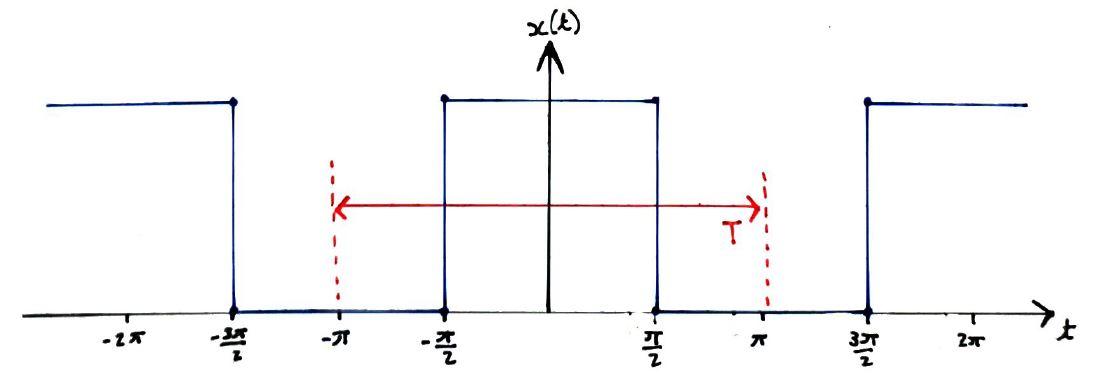
\includegraphics[width=\textwidth]{images/lecture_4_square_wave.JPG}
    \caption{
      A square wave signal of period $2\pi$ and duty cycle of $0.5$.
    }
    \label{fig::lecture_4_square_wave}
  \end{figure}
  %
  We see that it is periodic with period $T = 2\pi$, and be extension its
  angular frequency is $\omega_0 = \frac{2\pi}{T} = 1$. The zeroth spectral
  coefficient is given by the integral of the signal over its time period,
  %
  \begin{displaymath}
    a_0 = \frac{1}{T}\int_0^T\dx{t} x(t) = \frac{1}{2\pi}\times\pi = \frac{1}{2} \,.
  \end{displaymath}
  %
  For the remaining coefficients, we can integrate over any period of width $T$.
  Since the signal is even, we'll find it easier to integrate over $[-\pi,\pi]$.
  Upon further inspection, we find that this range can be reduced further to
  the non-zero regions, $[-\frac{\pi}{2},\frac{\pi}{2}]$. Now, performing the
  integration,
  %
  \begin{align*}
    a_k &= \frac{1}{2\pi}\int_{-\frac{\pi}{2}}^{\frac{\pi}{2}} \dx{t}\ex{-\im kt}
    = \left.\frac{1}{2\pi}\frac{-1}{\im k}\ex{-\im kt}\right|_{-\frac{\pi}{2}}^{\frac{\pi}{2}} \\
    &= -\frac{1}{2\pi\im k}\left(\ex{-\im k\frac{\pi}{2}} - \ex{\im k\frac{\pi}{2}}\right)
    = \frac{1}{2\pi\im k}\left(\ex{\im k\frac{\pi}{2}} - \ex{-\im k\frac{\pi}{2}}\right)
    = \frac{\sin(k\frac{\pi}{2})}{\pi k} \\
    &= \frac{1}{2}\sinc\left(\frac{k\pi}{2}\right) \,,
  \end{align*}
  %
  where we have introduced the function $\sinc = \frac{\sin(x)}{x}$. Consequently,
  we can write the first few spectral coefficients,
  %
  \begin{displaymath}
    a_1 = \frac{\sin\left(\frac{\pi}{2}\right)}{\pi} = \frac{1}{\pi}, \quad
    a_2 = \frac{\sin(\pi)}{2\pi} = 0, \quad
    a_3 = \frac{\sin\left(\frac{3\pi}{2}\right)}{3\pi} = -\frac{1}{3\pi}, \quad\hdots \,.
  \end{displaymath}
\end{exmp}
%
It will be useful to have some intuition for how the $\sinc$ function looks. It is
graphed in Figure \ref{fig::lecture_4_sinc}.
%
\begin{figure}[!htb]
  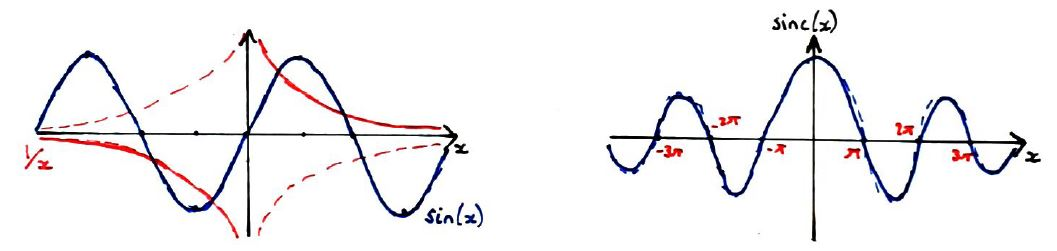
\includegraphics[width=\textwidth]{images/lecture_4_sinc.JPG}
  \caption{
    The $\sinc$ function. The important features worth keeping in mind are
    that at $\sinc(x) = 1$ at $x=0$, and the zeroes of $\sinc$ occur at
    integer multiples of $\pi$.
  }
  \label{fig::lecture_4_sinc}
\end{figure}

\subsection{Validity of the Fourier Series}
%
There are several types of function where the Fourier series doesn't really work. These
are summarised by the \textbf{Dirichlet conditions} for a real-valued periodic function. If these
conditions are satisfied, then the Fourier series converges absolutely to the
function to which it is derived.
%
\begin{enumerate}
\item The function must be square-integrable, i.e. $\int \dx{t}|x(t)|^2 < \infty$.
\item There must be a finite number of minima and/ or maxima.
\item The function must contain a finite number of discontinuities.
\end{enumerate}
%
It is interesting to consider what the Fourier series does at a discontinuity,
since it is formed by an infinite number of smooth basis functions. The Fourier
series converges absolutely at every continuous point, while it converges to the
average value of the function at a discontinuity. To see this, let's consider Figure \ref{fig::lecture_4_gibbs}.
At each discontinuity, the Fourier series yields zero, the average value of the function
at that point. Note also the overshoot in the Fourier series, referred to as the \textbf{Gibbs
Phenomenon}. This overshoot can never be less that roughly $9\%$ the height of the
discontinuity. The oscillations are referred to as \textbf{ringing artifacts} and the
continual overshooting/ undershooting of the desired value is termed \textbf{clipping}. 
%
\begin{figure}[!htb]
  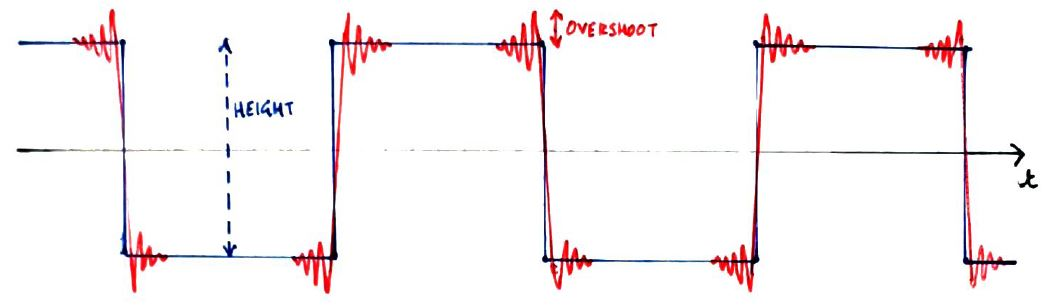
\includegraphics[width=\textwidth]{images/lecture_4_gibbs.JPG}
  \caption{
    A finite Fourier series representation of a signal. The Gibbs Phenomenon
    is clearly visible at the discontinuities.
  }
  \label{fig::lecture_4_gibbs}
\end{figure}


\subsection{Properties of the Fourier Series}
%
Suppose we have a periodic signal $x(t)$ with period $T$, whose Fourier series is given by
$\{a_k\}$. Then:
%
\begin{enumerate}
\item (\textbf{Linearity}) Given the signals $x(t) \Leftrightarrow \{a_k\}$ and
  $y(t) \Leftrightarrow \{b_k\}$, then
  %
  \begin{displaymath}
    \alpha x(t) + \beta y(t) \Leftrightarrow \{\alpha a_k + \beta b_k\} \,.
  \end{displaymath}
  %
\item (\textbf{Time Shifting}) For $x(t) \Leftrightarrow \{a_k\}$ and
  $y(t) = x(t-t_0)$, then
  %
  \begin{displaymath}
    y(t) \Leftrightarrow \{a_k\ex{-\im k\omega_0t_0}\} \,,
  \end{displaymath}
  %
  i.e. the magnitudes of the coefficients don't change, but the phases do.
\item (\textbf{Differentiation}) For $x(t) \Leftrightarrow \{a_k\}$,
  $x^\prime(t) \Leftrightarrow \{\im k\omega_0 a_k\}$. This is easily shown by
  differentiating the complex exponential basis function.
\item (\textbf{Parseval's Theorem}) There is the same amount of power in both time
  and frequency domains (i.e. no information loss),
  %
  \begin{displaymath}
    \frac{1}{T}\int_0^T \dx{t} |x(t)|^2 = \sum_{k=-\infty}^\infty |a_k|^2 \,.
  \end{displaymath}
  %
\item (\textbf{Convolution}) For the signals $x(t) \Leftrightarrow \{a_k\}$ and
  $y(t) \Leftrightarrow \{b_k\}$,
  %
  \begin{displaymath}
    x(t)y(t) \Longleftrightarrow \sum_{m=-\infty}^\infty a_m b_{k-m} = a * b \,,
  \end{displaymath}
  %
  or conversely
  %
  \begin{displaymath}
    x* y = \int_0^T \dx{\tau} x(\tau)y(t-\tau) \Longleftrightarrow Ta_kb_k \,.
  \end{displaymath}
  %
  In other words, convolution in one domain is multiplication in the other. 
\end{enumerate}
